\section{Large-scale problems} \label{section_71}

In this chapter, we consider the notion of \emph{decomposition}, which consists of a general term used in the context of mathematical programming to refer to solution methods that utilise some separability mechanism to more efficiently solve large-scale problems.

In general, decomposition methods are based on the premise that it is more efficient, under a computational standpoint, to repeatedly resolve a (collection of) smaller instances of a problem than to solve the full-scale original problem. More recently, with the widespread adoption of multithreaded processors and computing clusters with multiple nodes, decomposition methods have become attractive as parallelisation strategies, which can yield considerable computational savings. 

There are mainly two classes of decomposition methods. The first class utilises the explicit representation of polyhedral sets, as stated in Theorem \ref{p1c6:thm:resolution_theorem}, to iteratively reconstruct the full-scale problem, with the hope that the structure containing the optimal vertex will be successfully reconstructed before all of the problem itself is reconstructed. It turns out that this is the case in many applications, which is precisely the feature that renders these methods very efficient in some contexts. This is the class of methods we are going to analyse in this chapter, first the Dantzig-Wolfe decomposition and related column generation, and then its equivalent dual method, generally known as Benders' decomposition.

%TODO: Chp7: Add appropriate references.

The second class of methods utilises Lagrangian duality for obtaining separability. We will delay the presentation of this sort of approach to Part \ref{part_2}, when we discuss Lagrangian duality under the more general context of nonlinear programming problems.

In either case, decomposition methods are designed in a way that they seek to break problems into easier parts by removing linking elements. Specifically, let 
%
\begin{equation*}
	(P) : \mini \braces{c^\top x : x \in X},
\end{equation*}
%
where $X = \bigcap_{k=1}^K X_k,$ for some $K > 0$, and 
%
\begin{equation*}
	X_k = \braces{x^k \in \reals_+^{n_k} : D_kx_k = d_k}, \forall k \in \braces{1,\dots,K}.	
\end{equation*}
%
That is, $X$ is the intersection of $K$ standard-form polyhedral sets. Our objective is to devise a way to break into $K$ separable parts that can be solved separately and recombined as a solution for $P$. In this case, this can be straightforwardly achieved by noticing that $P$ can be equivalently stated as 
%
\begin{center}
    \begin{tabular}{rcccc}
	$(P): \maxi_x$ & $c_1^\top x_1$ & $+\dots+$ & $c_K^\top x_K$ & \\
	        $\st$  & $D_1x_1$ &           &          & $= d_1$ \\
	               &          & $\ddots$  &          & $\vdots$ \\
	               &          &           & $D_Kx_K$ & $= d_K$ \\
	               &  $x_1$,  & $\dots$,  & $x_K$    & $\in \reals^n_+$ 
	\end{tabular}
\end{center}
%
has a structure that immediately allows for separation. That is, $P$ could be solved as $K$ independent problems 
%
\begin{equation*}
	P_k : \mini \braces{c_k^\top x_k : x_k \in X_k}	
\end{equation*}
%
in parallel and then combine their individual solutions onto a solution for $P$, simply by making $\overline{x} = [x_k]_{k=1}^K$ and $c^\top \overline{x} = \sum_{i=1}^K c_k^\top \overline{x}_k$. Notice that, if we were to assume that the solution time scales linearly (it does not; it grows faster than linear) and $K=10$, then solving $P$ as $K$ separated problems would be ten times faster (that is not true; there are bottlenecks and other considerations to take into account, but the point stands). 

Unfortunately, \emph{complicating structures} often compromise this natural separability, preventing one from being able to directly exploit this idea. Specifically, two types of complicating structures can be observed. The first is of the form of \emph{complicating constraint}. That is, we observe that a constraint is such that it connects variables from (some of) the subsets $X_k$. In this case, we would notice that $P$ has an additional constraint of the form
%
\begin{equation*}
	A_1x_1 + \dots + A_Kx_K = b,
\end{equation*}
%
which precludes separability, since the problem structure becomes
% 
\begin{center}
	\begin{tabular}{rcccc}
	    $P':  \maxi_x$ & $c_1^\top x_1$ & $+\dots+$ & $c_K^\top x_K$ & \\
	            $\st$  & $A_1x_1$ & $+\dots+$ & $A_Kx_K$ & $=b$ \\
	                   & $D_1x_1$ &           &          & $= d_1$ \\
	                   &          & $\ddots$  &          & $\vdots$ \\
	                   &          &           & $D_Kx_K$ & $= d_K$ \\
	                   &  $x_1$,  & $\dots$,  & $x_K$ & $\in \reals^n_+$. 
	\end{tabular}
\end{center}

The other type of complicating structure is the case in which the same set of decision variable is present in multiple constraints, or multiple subsets $X_k$. In this case, we observe that variables of a subproblem $k \in \braces{1,\dots,K}$ has nonzero coefficient in another subproblem $k' \neq k$, $k' \in \braces{1,\dots,K}$. Hence, problem $P$ takes the form of
%
\begin{center}
	\begin{tabular}{rccccc}
	$P''$ : $\maxi_x$ & $c_0^\top x_0 +$ &  $c_1^\top x_1$ & $+\dots+$ & $c_K^\top x_K$ & \\
        $\st$  & $A_1x_0+$ & $D_1x_1$ &           &          & $= d_1$ \\
               & $\vdots$  &          & $\ddots$  &          & $\vdots$ \\
               & $A_Kx_0+$ &          &           & $D_Kx_K$ & $= d_K$ \\
               & $x_0,$    &  $x_1$,  & $\dots$,  & $x_K$    & $\in \reals^n_+$. 
	\end{tabular}
\end{center}
%
The challenging aspect is that a specific method becomes more suitable depending on the complicating structure. Therefore, being able to identify these structures is one of the key success factors in terms of the chosen method's performance. As a general rule, problems with complicating constraints (as $P'$) are suitable to be solved by a delayed variable generation method such as column generation. Analogously, problems with complicating variables ($P''$) are better suited for employing delayed constraint generation methods such as Benders decomposition. 

The development of professional-grade code employing decomposition methods is a somewhat recent occurrence. The commercial solver CPLEX offers a Benders decomposition implementation that requires the user to specify the separable structure. On the other hand, although there are some available frameworks for implementing column generation-based methods, these tend to be more ad hoc occurrences yet often reap impressive results.  


\section{Dantzig-Wolfe decomposition and column generation*} \label{section_72}

Before we move forward, we need to discuss some technical results that will be useful for describing the Dantzig-Wolfe and Benders decomposition methods. Those are results mostly based on the notion of linear duality from Chapters \ref{chapter_5} and \ref{chapter_6}.

\subsection{Resolution theorem}

%Lastly, we present a result that will be the foundation for our discussion in the next chapter. Specifically, we will see how we can use a presentation of the polyhedral set $P$ purely based on extreme points and extreme rays to devise solution strategies that can be more efficient for large-scale linear programming problems. 

%For now, let us concentrate on this alternative representation. 
%Basically, p
A polyhedral set $P$ in standard form can be represented in two manners: either by (i) a finite set of linear constraints; or (ii) by combinations of its extreme points and extreme rays. Clearly, the first representation is far more practical than the second. That is, the second representation is an \emph{explicit} representation that would require knowing beforehand each extreme point and extreme ray forming the polyhedral set. 

Notice that the first representation, which we have relied on so far, has extreme points and extreme rays only implicitly represented. However, we will see that this explicit representation has an important application in the devising of alternative solution methods for large-scale linear programming problems. This fundamental result is stated in Theorem \ref{p1c7:thm:resolution_theorem}. 

\begin{theorem}[Resolution theorem]\label{p1c7:thm:resolution_theorem}
	Let $P = \braces{x \in \reals^n : Ax \geq b}$ be a nonempty polyhedral set with at least one extreme point. Let $\braces{x_i}_{i=1}^k$ be the set with all extreme points, and $\braces{w}_{j=1}^r$ be the set of all extreme rays of $P$. Then $P = Q$, where 
	\begin{equation*}
		Q = \braces{\sum_{i=1}^k \lambda_i x^i + \sum_{j=1}^r \theta_jw^j : \lambda_i \geq 0, \ \theta_j \geq 0, \ \sum_{i=1}^k \lambda_i =1}.
	\end{equation*}
\end{theorem}

%TODO: Chp7: Include proof for the resolution theorem

Theorem \ref{p1c7:thm:resolution_theorem} has an important consequence, as it states that bounded polyhedra, i.e., a polyhedral set that has no extreme rays, can be represented by the convex hull of its extreme points. For now, let us look at an example that illustrates the concept.

Consider the polyhedral set $P$ given by
%
\begin{equation*}
	P = \braces{x_1 - x_2 \geq -2; x_1 + x_2 \geq 1, x_1,x_2 \geq 0}.
\end{equation*}
%
The recession cone $C = {\bf recc}(P)$ is described by $d_1 - d_2 \geq 0$, $d_1 + d_2 \geq 0$ (from $Ad =0$), and $d_1, d_2 \geq 0$, which can be simplified as 
%
\begin{equation*}
	C = \braces{(d_1, d_2) \in \reals^2 : 0 \leq d_2 \leq d_1}.
\end{equation*}
%
We can then conclude that the two vectors $w^1 = (1,1)$ and $w_2 = (1,0)$ are extreme rays of $P$. Moreover, $P$ has three extreme points: $x_1 = (0,2)$, $x_2 = (0,1)$, and $x_3 = (1,0)$.

Figure \ref{p1c7:fig:resolution_example} illustrates what is stated in Theorem \ref{p1c7:thm:resolution_theorem}. For example,  a representation for the point $y = (2,2) \in P$ is given by
%
\begin{equation*}
	y = \begin{bmatrix} 2 \\ 2
		\end{bmatrix}= \begin{bmatrix} 0 \\ 1
		\end{bmatrix} + \begin{bmatrix} 1 \\ 1
		\end{bmatrix} + \begin{bmatrix} 1 \\ 0
		\end{bmatrix}, 	
\end{equation*}
%
that is, $y = x^2 + w^1 + w^2$. Notice, however, that $y$ could also be represented as 
%
\begin{equation*}
	y = \begin{bmatrix} 2 \\ 2
		\end{bmatrix}= \frac{1}{2}\begin{bmatrix} 0 \\ 1
		\end{bmatrix} + \frac{1}{2}\begin{bmatrix} 1 \\ 0
		\end{bmatrix} + \frac{3}{2}\begin{bmatrix} 1 \\ 1
		\end{bmatrix}, 	
\end{equation*}
%
with then $y = \frac{1}{2}x^2 + \frac{1}{2}x^3 + \frac{3}{2}w^1$. Notice that this imply that the representation of each point is not unique.

\begin{figure}[h]
	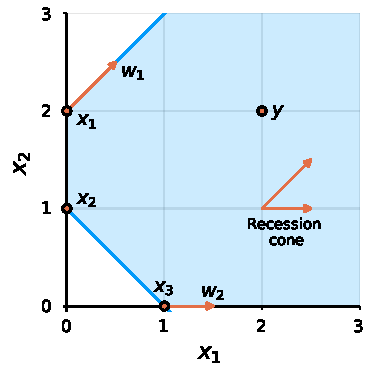
\includegraphics{part_1/chapter_7/figures/Figure1.pdf}
	\caption{Example showing that every point of $P = \braces{x_1 - x_2 \geq -2; x_1 + x_2 \geq 1, x_1,x_2 \geq 0}$ can be represented as a convex combination of its extreme point and a linear combination of its extreme rays} \label{p1c7:fig:resolution_example}
\end{figure}


\subsection{Dantzig-Wolfe decomposition}

We start with the Dantzig-Wolfe decomposition, which consists of an alternative approach for reducing memory requirements when solving large-scale linear programming problems. Then, we show how this can be expanded further with the notion of delayed variable generation to yield a truly decomposed problem.

As before, let $P_k = \braces{x_k \geq 0 : D_kx_k = d}$, with $P_k \neq \emptyset$ for $k \in \braces{1,\dots,K}$. Then, the problem $P$ can be reformulated as:
%
\begin{align*}
	\mini \ & \sum_{k = 1}^K c_k ^\top x_k 	\\
	\st & \sum_{k=1}^K A_k x_k = b \\
	& x_k \in P_k, \ \forall k \in \braces{1,\dots,K}. 
\end{align*}
%
Notice that $P$ has a complicating constraint structure, due to the constraints $\sum_{k=1}^K A_k x_k = b$. In order to devise a decomposition method for this setting, let us first assume that we have available for each of the sets $P_k$, $k \in \braces{1,\dots,K}$, (i) all extreme points, represented by $x_k^j$, $\forall j \in J_k$; and (ii) all extreme rays $w_k^r$, $\forall r \in R_k$. As one might suspect, this is in principle a demanding assumption, but one that we will be able to drop later on.

Using the Resolution theorem (Theorem \ref{p1c7:thm:resolution_theorem}), we know that any element of $P_k$ can be represented as 
%
\begin{equation} \label{p1c7:eq:resolution_representation}
	x_k = \sum_{j \in J_k} \lambda_k^j x_k^j + \sum_{r \in R_k} \theta_k^r w_k^r, 	
\end{equation}
%
where $\lambda_k^j \geq 0$, $\forall j \in J_k$, are the coefficients of the convex combination of extreme points, meaning that we also observe $\sum_{j \in J_k} \lambda_k^j = 1$, and $\theta_k^r \geq 0$, $\forall r \in R_k$, are the coefficients of the conic combination of the extreme rays.

Using the identity represented in \eqref{p1c7:eq:resolution_representation}, we can reformulate $P$ onto the \emph{main problem} $P_M$ as follows.
%
\begin{align} 
	(P_M) : \mini \ & \sum_{k =1}^K \left(\sum_{j \in J_k} \lambda_k^jc_k ^\top x^j_k   + \sum_{r \in R_k} \theta_{k}^rc_k^\top w_k^r \right)	\nonumber\\
	\st & \sum_{k = 1}^K \left(\sum_{j \in J_k}\lambda_k^j A_k x_k^j + \sum_{r \in R_k} \theta_k^r A_k w_k^r\right) = b \label{p1c7:eq:pm_const}\\
	& \sum_{j \in J_k}\lambda_k^j = 1, \ \forall k \in \braces{1, \dots, K} \label{p1c7:eq:cc_const}\\
	& \lambda_k^j \geq 0,  \theta_k^r \geq 0, \forall j \in J_k, r \in R_k, k \in \braces{1, \dots, K}. \nonumber 
\end{align}
%
Notice that \eqref{p1c7:eq:pm_const} and \eqref{p1c7:eq:cc_const} can be equivalently represented as
%
\begin{equation*}
	\sum_{k \in K}\left(\sum_{j \in J_k}\lambda_k^j \begin{bmatrix} A_kx_k^j \\ e_k\end{bmatrix} + \sum_{r \in R_k}\theta_k^r \begin{bmatrix} A_kw_k^r \\ 0\end{bmatrix}\right) = \begin{bmatrix} b \\ 1\end{bmatrix},
\end{equation*}
%	  	   
where $e_k$ is the unit vector (i.e., with 1 in the $k^\text{th}$ component, and $0$ otherwise). Notice that $P_M$ has as many variables as the number of extreme points and extreme rays of $P$, which is likely to be prohibitively large.

However, we can still solve it if we use a slightly modified version of the revised simplex method. To see that, let us consider that $b$ is a $m$-dimensional vector. Then, a basis for $P_M$ would be of size $m + K$, since we have the original $m$ constraints plus one for each convex combination (arising from each subproblem $k \in K$). This means that we are effectively working with $(m + K) \times (m + K)$ matrices, i.e., the basic matrix $B$ and its inverse $B^{-1}$. Another element we need is the vector of simplex multipliers $p$, which is a vector of dimension $(m + K)$.

The issue with the representation adopted in $P_M$ arises when we are required to calculate the reduced costs of \emph{all} the nonbasic variables, since this is the critical issue for its tractability. That is where the method provides a clever solution. To see that, notice that the vector $p$ is formed by components $p^\top = (q, r_1, \dots, r_K)^\top$, where $q$ represent the $m$ dual variables associated with \eqref{p1c7:eq:pm_const}, and $r_k$, $\forall k \in \braces{1,\dots,K}$, are the dual variables associated with \eqref{p1c7:eq:cc_const}. 

The reduced costs associated with the extreme-point variables $\lambda_k^j$, $j \in J_K$, is given by
%
\begin{equation}
	c_k^\top x_k^j - [q^\top ~ r_1 ~ \dots ~ r_K]	\begin{bmatrix} A_k x_k^j \\ e_k \end{bmatrix} = (c_k^\top - q^\top A_k)x_k^j - r_k.
\end{equation}
%
Analogously, the reduced cost associated with extreme-ray variables $\theta_k^r$, $r \in R_k$, is
\begin{equation}
	c_k^\top w_k^r - [q^\top ~ r_1 ~ \dots ~ r_K]	\begin{bmatrix} A_k w_k^r \\ 0 \end{bmatrix} = (c_k^\top - q^\top A_k)w_k^r.
\end{equation}
%
The main difference is how we assess the reduced costs of the non-basic variables. Instead of explicitly calculating the reduced costs of all variables, we instead rely on an optimisation-based approach to consider them only \emph{implicitly}. For that, we can use the subproblem 
%
\begin{align*}
	(S_k):  \mini_x \overline{c}_k = \ & (c_k^\top - q^\top A_k)x_k \\
	\st & x_k \in P_k,			
\end{align*} 
%
which can be solved in parallel for each subproblem $k \in \braces{1,\dots,K}$. The subproblem $S_k$ is known as the \emph{pricing problem}. For each subproblem $k = 1, \dots, K$, we have the following cases.

 We might observe that $\overline{c}_k = -\infty$. In this case, we have found an \emph{extreme ray} $w_k^r$ satisfying $(c_k^\top - q^\top A_k)w_k^r < 0$. Thus, the reduced cost of the associated extreme-ray variable $\theta_k^r$ is negative. 

If that is the case, we must generate the column
%
\begin{equation*}
	\begin{pmatrix}
		A_kw_k^r \\ 0
	\end{pmatrix}
\end{equation*}
%
associated with $\theta_k^r$ and make it enter the basis.		

Otherwise, being $S_k$ bounded, i.e., $\overline{c}_k < \infty$, two other cases can occur. The first is the case in which $\overline{c}_k < r_k$. Therefore, we found an extreme point $x_k^j$ satisfying $(c_k^\top - q^\top A_k)x_k^j - r_k < 0$. Thus, the reduced cost associated with the extreme-point variable $\lambda_k^j$ is negative and, analogously, we must generate the column
%
\begin{equation*}
	\begin{pmatrix}
		A_kx_k^j \\ e_k
	\end{pmatrix}
\end{equation*}
%
associated with $\lambda_k^j$ and make it enter the basis.

The last possible case is when we observe that $r_k < \overline{c}_k < \infty$. In this case, the pricing problem could not identify a beneficial variable to be made basic, and therefore there is not an extreme point or ray with negative reduced cost for subproblem $k$. If this condition holds for all $k = 1, dots, K$, then all necessary extreme points and rays to characterise the region where the optimal extreme point lies (or one of the extreme points, in the case of multiple solutions) have been found and the optimal solution can be recovered. 

Algorithm \ref{p1c7:alg:DW} summarises the Dantzig-Wolfe method. The two most remarkable features of the method are (i) the fact that columns are not explicitly represented, but generated ``on demand'' and (ii) the fact that the pricing problem requires the solution of another linear programming problem. Analogously to the simplex method, it might be necessary to employ a ``Phase 1'' approach to obtain an initial basis to start the algorithm.

\begin{algorithm}[h]
\caption{Dantzig-Wolfe decomposition} \label{p1c7:alg:DW}
\begin{algorithmic}[1] %line numbering frequency. 
	\State {\bf initialise.} 
	Let $B$ be a BFS for $P_M$ and set $l \gets 0$. 
	\Repeat 
	   \For {$k \in \braces{1,\dots,K}$} 
	        \State solve $S_k$ and let $\overline{c}_k = \min_x \braces{S_k}$
	        \If{$\overline{c}_k  = -\infty$} 
	        	\State obtain extreme ray $w_k^r$ and make $R_k^l = R_k^l \cup \braces{w_k^r}$.
	        	\State generate column $(A_kw_k^r, 0)$ to become basic.
	        \ElsIf {$\overline{c}_k < r_k < \infty$}
	        	\State obtain extreme point $x_k^j$ and make $J_k^l = J_k^l \cup \braces{x_k^j}$.
	        	\State generate column $(A_kx_k^j, e_k)$ to become basic.
	        \EndIf  
	    \EndFor
			\State select one of the generated columns to replace one of the columns of $B$ and update $B$ accordingly. 
	    \State $l \gets l + 1$.            	
		\Until{$\overline{c}_k  > r_k$ for all $k \in \braces{1,\dots,K}$} 
	\State {\bf return} $B$
\end{algorithmic}  
\end{algorithm}

Under a theoretical standpoint, the Dantzig-Wolfe method is equally efficient as the revised simplex method. There are however two settings where the decomposition is most favourable. The first, consists of applications in which the pricing problem can be solved in a closed-form, without invoking a method to solve an additional linear programming subproblem. There are a few examples in which this happens to be the case and certainly many others yet to be discovered.

Secondly, the memory requirements of the Dantzig-Wolfe decomposition makes it an interesting approach for very large-scale problems. The original simplex method requires an amount of memory space that is $O((m + K \times m_0)^2)$, where $m_0$ is the number of rows of $D_k$, for $\forall k \in \braces{1,\dots, K}$. This is essentially the size of the inverse basic matrix $B^{-1}$. In contrast, the Dantzig-Wolfe reformulation requires $O((m + K)^2) + K \times O(m_0^2)$ of memory space, with the first term referring to the main problem inverse basic matrix and the second to the pricing problems basic matrices. For example, for a problem in which $m = m_0$ and much larger than, say, $K=10$, this implies that the memory space required by the Dantzig-Wolfe reformulation is 100 times smaller, which can substantially enlarge the range of large-scale problems that can be solved for the same amount of computational resources available.


\subsection{Delayed column generation}
 
The term column generation can also refer to a related, and perhaps more widely known, variant of the Dantzig-Wolfe decomposition. In that, the main problem $P_M$ is also repeatedly solved, each time being incremented by an additional variable (or variables) associated with the column(s) identified with negative reduced costs in the pricing problem $S_k$, $k \in \braces{1,\dots,K}$. This is particularly useful for problems with exponentially increasing number of variables, or with a large number of variables associated with the complicating constraints (i.e., when $m$ is a large number).

\begin{algorithm}[h]
    \caption{Column generation algorithm} \label{p1c7:alg:CG}
    \begin{algorithmic}[1] %line numbering frequency. 
    \State {\bf initialise.} 
    Let $\tilde{X}_k \subset X_k$, for $k \in \braces{1,\dots,K}$, and set
    $l \gets 0$. 
    	\Repeat \label{Alg2:loop}
        \State solve $P_M^l$ to obtain $\lambda^{*l} = (\lambda_1^{*l},\dots, \lambda_K^{*l})$ and duals $(q^{*l}, \braces{r_k^{*l}}_{k=1}^K)$.
        \For {$k \in \braces{1,\dots,K}$} 
            \State solve the pricing problem
            $$\overline{x}^{*l}_k \gets \argmin \braces{c_k^\top x_k - q^{*l}(A_kx_k) - r^{*l}_k : x_k \in P_k}.
            $$
            \If{$\overline{c}_k = c_k^\top \overline{x}^{*l}_k - q^{*l}(A_k\overline{x}^{*l}_k) < r^{*l}_k$} $\tilde{X}_k \gets \tilde{X}_k \cup \braces{\overline{x}^{*l}_k}$ \label{p1c7:alg:CGcolgen}
            \EndIf  
        \EndFor
        \State $l \gets l + 1$.
    	\Until{$\overline{c}_k  > r_k$ for all $k \in \braces{1,\dots,K}$} 
    \State {\bf return} $\lambda^{*l}$.
    \end{algorithmic}
\end{algorithm}

The (delayed) column generation method is presented in Algorithm \ref{p1c7:alg:CG}. Notice in Line \ref{p1c7:alg:CGcolgen} the step that is generating new columns in the main problem $P_M$, represented in the statement $\tilde{X}_k \gets \tilde{X}_k \cup \braces{\overline{x}^{*l}_k}$. That is precisely when new variables $\lambda_k^{t}$ are introduced in the $P_M$ with coefficients represented by the column
%
\begin{equation*}
	\begin{pmatrix}
            c_k\overline{x}_k^{*l}\\
            A_k\overline{x}_k^{*l}\\
            e_k
    \end{pmatrix}.
\end{equation*}

Notice that the unbounded case is not treated to simplify the pseudocode, but could be trivially adapted to return extreme rays to be used in $P_M$, like the previous variant presented in Algorithm \ref{p1c7:alg:DW}. Also, notice that the method is assumed to be initialised with a collection of columns (i.e., extreme points) $\tilde{X}_k$, which can normally be obtained from inspection or using a heuristic method.

We finalise showing that the Dantzig-Wolfe and column generation methods can provide information related to its own convergence. This means that we have access to an optimality bound that can be used to monitor the convergence of the method and allow for a preemptive termination given an acceptable tolerance. This bounding property is stated in Theorem \ref{p1c7:thm:CG_bound}.

\begin{theorem} \label{p1c7:thm:CG_bound}
	Suppose $P$ is feasible with finite optimal value $z$. Let $\overline{z}$ be the optimal cost associated with $P_M$ at a given iteration $l$ of the Dantzig-Wolfe method. Also, let $r_k$ be the dual variable associated with the convex combination of the $k^\text{th}$ subproblem and $z_k$ its optimal cost. Then
		%
		\begin{equation*}
			z + \sum_{k=1}^K (z_k - r_k) \leq z \leq \overline{z}.	
		\end{equation*}
\end{theorem}

\begin{proof}
	
	We know that $z \leq \overline{z}$, because a solution for $P_M$ is primal feasible and thus feasible for $P$.
	
	Now, consider the dual of $P_M$
	%
	\begin{align*}
		(D_M): ~\maxi \ & q^\top b + \sum_{k=1}^K r_k \\
		\st & q^\top A_k x_k^j + r_k \leq c_k^\top x_k^j, \ \forall j \in J_k, \forall k \in \braces{1,\dots, K} \\
		& q^\top A_kw_k^r \leq c_k^\top w_k^r, \ \forall r \in R_k, \forall k \in \braces{1,\dots, K} \\ 
	\end{align*}
	%
	We know that strong duality holds, and thus $z = q^\top b + \sum_{k=1}^K r_k $ for dual variables $(q, r_1, \dots, r_K)$. 
	
	Now, since $z_k$ are finite, we have $\min_{j \in J_k}(c_k^\top x_k^j - q^\top A_k x_k^j) = z_k$ and $\min_{r \in R_k}(c_k^\top w_k^r - q^\top D_k w_k^r) \geq 0$, meaning that $(q, z_1, \dots, z_K)$ is feasible to $D_M$. By weak duality, we have that
	%
	\begin{equation*}
		z \geq q^\top b + \sum_{k=1}^K	z_k = q^\top b + \sum_{k=1}^K r_k + \sum_{k=1}^K (z_k - r_k) = z + \sum_{k=1}^K (z_k - r_k). \qedhere	
	\end{equation*}
\end{proof}


\section{Benders decomposition}

Benders decomposition is an alternative decomposition method, suitable for settings in which \emph{complicating variables} are present. Differently than the Dantzig-Wolfe decomposition, the method presumes from the get-go the employment of delayed constraint generation. 

Benders decomposition has made significant inroads into practical applications. Not only is it extensively used in problems related to multi-period decision-making under uncertainty, but it is also available in the commercial solver CPLEX to be used directly, only requiring the user to indicate (or annotate) which are the complicating variables. 


\subsection{Parametric optimisation problems} \label{section_731}

Before we proceed, let us develop the idea of having optimisation problems stated as functions of the input data. Specifically, let 
%
\begin{equation*}
	P(b) = \braces{x \in \reals^n : Ax = b, x \geq 0}
\end{equation*}
%
be defined as a function of the input vector $b \in \reals^m$. That is, $P(b)$ is the set of feasible solutions when the right-hand side is set to $b$. Then, let $S = \braces{b \in \reals^m : P(b) \neq \emptyset}$ be the set of all vectors $b$ for which $P$ has at least one feasible solution. Being so, we can restate the set $S$ as 
%
\begin{equation*}
	S = \braces{Ax : x \ge 0}.
\end{equation*}
%
That is, the set $S$ is formed by the conic combination of the columns of $A$ for which $x$ is nonnegative (or, in other words, that $P(b)$ is feasible). Also, notice that this is a convex set, as discussed in Section \ref{section_621}. For any $b \in S$, we can define the function
%
\begin{equation}
	F(b) = \min_x \braces{c^\top x : x  \in P(b)},	
\end{equation}
%
which takes as an argument $b$ and returns the optimal value of the parametrised optimisation problem. Notice that evaluating $F$ requires that an optimisation problem is solved.

Now, let us assume that the dual feasibility set 
%
\begin{equation*}
	S_D = \braces{p \in \reals^m : p^\top A \le c}	
\end{equation*}
% 
is not empty. That implies that $F(b)$ is finite for every $b \in S$ since different $b$'s simply imply that different objective functions $p^\top b$ over $S_D$ are considered. Our main objective here is to understand the structure of the function $F: S \mapsto \reals$. 

Let $\overline{b} \in S$ be a particular $b$. Suppose that there exists a nondegenerate optimal BFS $x_B$ with basis $B$. Then, we have that $x_B = B^{-1}\overline{b}$, $F(\overline{b}) = c_B^\top x_B =  c_B^\top B^{-1}\overline{b}$ and that all reduced costs are nonnegative. 

Now, if we change $\overline{b}$ to $b$ such that the difference is sufficiently small, $B^{-1}\overline{b}$ remains positive and, consequently, $x_B$ remains a basic feasible solution. Furthermore, since $b$ does not affect the reduced costs (recall that our optimality condition is given by $\overline{c} = c^\top - c_B ^\top B^{-1}A \ge 0$), they remain nonnegative. Notice that this is the same argument we used in Section \ref{section_613} when we discussed changes in the input data in the context of sensitivity analysis.

The optimal value $F(b)$ associated with this new $b$ sufficiently close to $\overline{b}$   
%
\begin{equation*}
	F(b) - F(\overline{b})= c_B B^{-1}(b - \overline{b}) = p^\top (b - \overline{b}) 
\end{equation*}
%
where $p = c_B B^{-1}$ is the optimal solution of the dual problem 
%
\begin{align*}
	\maxi & p^\top b \\
	\st   & p^\top A \le c.
\end{align*}
%
This allows us to observe two important characteristics of $F$. First, in the vicinity of $\overline{b}$, $F(b)$ is a linear function of $b$, Also, $p$ represents a \emph{gradient} of $F$. This, again, is an alternative view to the conclusions we drew earlier in Section \ref{section_613}, and, in a way, further strengthens the idea of the optimal dual variables $p$ representing marginal values regarding changes in the components of $b$.

With the above, we can formalise an important result regarding the convexity of the function $F(b)$.

\begin{theorem}[Convexity of $F(b)$]
	The optimal value function $F(b)$ is convex in $b$ on the set $S$.
\end{theorem}

\begin{proof}

	Let $b^i \in S$ and $x^i$ be their associated optimal solution, for $i = 1,2$. Thus, $F(b^i) = c^\top x^i$, for $i=1,2$. Let $\lambda \in [0,1]$. The vector $\overline{x} = \lambda x^1 + (1-\lambda)x^2$ is nonnegative, and $A\overline{x} = \lambda b^1 + (1-\lambda)b^2$. Thus, $\overline{x}$ is a feasible solution when $b$ is set to $\lambda b^1 + (1-\lambda)b^2$. Therefore,
	%
	\begin{equation*}
		F(\lambda b^1 + (1-\lambda)b^2) \le c^\top \overline{x}	= \lambda c^\top x^1 + (1-\lambda) c^\top x^2 = \lambda F(b^1) + (1-\lambda) F(b^2),
	\end{equation*}
	%
	which is the definition of a convex function. The first inequality is valid because $\overline{x}$ is a feasible solution for when $b$ is set to $\lambda b^1 + (1-\lambda)b^2$.
\end{proof}


\subsection{Properties of the optimal value function $F(b)$} \label{section_732}

Let us again consider the dual problem $D$
%
\begin{align*}
	D: \maxi & p^\top b \\
	\st   & p^\top A \le c,
\end{align*}
%
which is again assumed to be feasible. For any $b$ in $S$, $F(b)$ is finite, and by strong duality (cf. Theorem \ref{p1c5:thm:strong_duality}), we have that $F(b) = p^\top b$. Because of our outstanding assumption that $A$ has $m$ linearly independent rows (and therefore, $m$ linearly independent columns), Theorem \ref{p1c3:thm:exist_extreme_point} guarantees that the feasible region of $D$ has at least one extreme point.

Let us suppose that we know all the extreme points $p^1, \dots, p^K$ of $D$. As the optimal solution for $D$ must be an extreme point, we can redefine $F$ as
%
\begin{equation} \label{p1c7:eq:function_F}
	F(b) = \max_{i = 1, \dots, K} (p^i)^\top b, \forall b \in S.
\end{equation}
%
Specifically, $F$ is the maximum of a finite collection of linear functions, and thus, piecewise linear. Furthermore, within the region where $F(b)$ is linear, or, as we have seen before, the change in $b$ is such that the corresponding optimal basis $B$ of the primal does not change, $F(b) = (p^i)^\top b$ where $p^i$ is the corresponding dual cost.

Finally, we must consider the lack of differentiability of $F$. Notice that specific values of $b$ will indicate the point at which the optimal basis $B$ changes, which implies a change in $p$. These ``junctions'' represent the points in which $D$ has multiple (i.e., not unique) solutions, which, as we have also seen, implies that the primal problem becomes degenerate.

Let us assume that we change $b$ in a particular way, i.e., $b = \overline{b} + \theta d$, where $\theta \in \reals$. We can then redefine $F$ by letting 
%
\begin{equation*}
	f(\theta) = F(\overline{b} + \theta d).
\end{equation*}
%
From \eqref{p1c7:eq:function_F}, we obtain
%
\begin{equation*}
	f(\theta) = \max_{i = 1, \dots, K} (p^i)^\top (\overline{b} - \theta d), \overline{b} + \theta d \in S
\end{equation*}
%
which represents the optimal cost as a function of the scalar $\theta$. In fact, $f(\theta)$ represents a section of the function $F$ in the direction given by the vector $d$, which is thus also piecewise linear and convex (and can be plotted). Figure \ref{p1c7:fig:b_function_theta} illustrates the function $f$ projected onto direction $d$ as a function of $\theta$.

\begin{figure}
	\begin{tikzpicture}
		\node (pic) at (0,0) {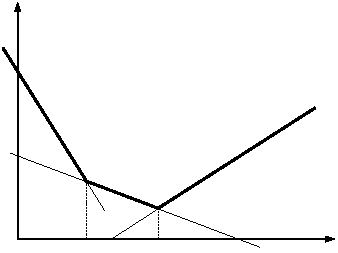
\includegraphics{part_1/chapter_7/figures/Figure2.pdf}};
		\node[right] (p1) at (-1.75,-0.25) {$(p^1)^\top (\overline{b} + \theta d)$};
		\node[right] (p2) at (0.5, -1.5) {$(p^2)^\top (\overline{b} + \theta d)$};
		\node[right] (p3) at (1.25,-0.6) {$(p^3)^\top (\overline{b} + \theta d)$};
		\node[below] (theta1) at (-1.4, -1.9) {$\theta_1$};
		\node[below] (theta2) at (-0.125, -1.9) {$\theta_2$};
		\node[below] (theta) at (2.7, -1.9) {$\theta$};
		\node[right] (f_theta) at (-2.5, 2) {$f(\theta)$};
	\end{tikzpicture}	
	\caption{The optimal cost function $F$ as a function of $b$ in the direction $d$. The feasibility set $S_D$ has three extreme points $p^1$, $p^2$, and $p_3$, each associated with a hyperplane $(p^i)^\top(\overline{b} + \theta d)$} \label{p1c7:fig:b_function_theta}
\end{figure}

To finalise, we return to one remaining issue associated with differentiability. Although $p$ can be seen as a gradient of $F(b)$ at $b$, we know that $F$ is not differentiable everywhere. To circumvent that, we require a generalisation of the the concept of gradients, which is given by the notion of subgradients. 

\begin{definition}
	Let $F$ be a convex function on the convex set $S$. Let $\overline{b} \in S$ The vector $p$ is a subgradient of of $F$ at $\overline{b}$ if
	\begin{equation}
		F(\overline{b}) + p^\top (b - \overline{b}) \le F(b), \forall b \in S.
	\end{equation}
\end{definition}

Figure \ref{p1c7:fig:b_function} illustrates the notion of a subgradient. Notice that, in general, the subgradient is a singleton, composed only of the gradient (or normal vector) of the hyperplane, which is given by the vector $p$. At the nondifferentiable points (the junctions), the subgradient comprises all hyperplanes defined between the two hyperplanes intersecting (or all nonnegative linear combinations of the normal vectors of the intersecting hyperplanes). For these values of $b$, we notice that the dual problem has multiple solutions, implying that the referring BFS to the primal problem is denegerate.   


The last result we need is to show that the optimal solution of the dual problem $p^*$ is in fact a subgradient of $F(\overline{b})$ at $\overline{b}$.

\begin{theorem}
	Suppose that the linear programming problem $P = \mini \braces{c^\top x : Ax = \overline{b}, x \ge 0}$ is feasible and the optimal cost is finite. Then, a vector $p \in \reals^m$ is an optimal solution to the dual problem if and only if it is a subgradient of the optimal value function $F$ at $\overline{b}$.
\end{theorem}

\begin{proof}
	Recall that $F$ is defined on the set $S = \braces{b \in \reals^m : P(b) \neq \emptyset}$, and that $P(b) = \braces{x \in \reals^n : Ax = b, x \geq 0}$. Suppose $p$ is an optimal solution to the dual problem $D$. Then, strong duality implies that $p^\top \overline{b} = F(\overline{b})$. Consider now an arbitrary $b \in S$. For any feasible solution $x \in P(b)$, we have from weak duality that 
	\begin{equation*}
		p^\top b \le c^\top x \Rightarrow p^\top b \le \min_{x \in P(b)} c^\top x = F(b).
	\end{equation*}
	Notice that this implies that $p^\top b - p^\top \overline{b} \le F(b) - F(\overline{b})$, which in turn yields that $p$ is a subgradient of $F$ at $\overline{b}$ since it rearranges to
	\begin{equation*}
		F(\overline{b}) + p^\top (b - \overline{b}) \le F(b).
	\end{equation*}
	Let us consider the converse. Assume that $p$ is a subgradient of $F$ at $\overline{b}$. Thus, we have 
	\begin{equation}
		F(\overline{b}) + p^\top (b - \overline{b}) \le F(b), \ \forall b \in S. \label{p1c7:eq:subgradient_proof}
	\end{equation}
	Let choose an $x \ge 0$, and let $b = Ax$, meaning that $x \in P(b)$ and that $F(b) \le c^\top x$. Using \eqref{p1c7:eq:subgradient_proof}, we obtain
	\begin{equation*}
		p^\top Ax = p^\top b \le F(b) - F(\overline{b}) + p^\top \overline{b} \le c^\top x - F(\overline{b}) + p^\top \overline{b}.
	\end{equation*}
	Since $x \ge 0$, this implies that $p^\top A \le c$, showing that $p$ is a dual feasible solution. Also, for $x = 0$, we obtain $F(\overline{b}) \le p^\top \overline{b}$. Now, using weak duality, we have that a dual feasible solution $p'$ satisfies $(p')^\top \overline{b} \le F(\overline{b})$. Combining the two, we show that $p$ is dual optimal, since
	\begin{equation*}
		(p')^\top \overline{b} \le  p^\top \overline{b}.
	\end{equation*}
\end{proof}

\begin{figure}[h]
	\begin{tikzpicture}
		\node (pic) at (0,0) {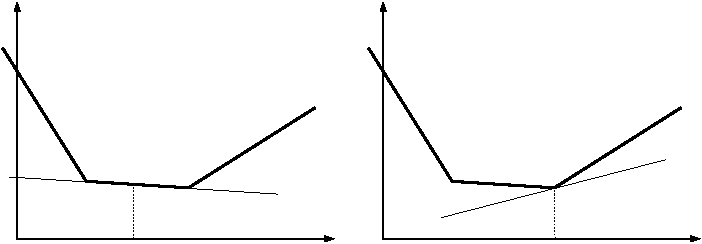
\includegraphics{part_1/chapter_7/figures/Figure3.pdf}};
		\node[right] (Fb1) at (-3,-1.5) {$F(\overline{b}) + p^\top(b - \overline{b})$};
		\node[right] (Fb2) at (4.6,-1) {$F(\overline{b}) + p^\top(b - \overline{b})$};
		\node[below] (b1) at (-3.7, -2) {$\overline{b}$};
		\node[below] (b2) at (3.4, -2) {$\overline{b}$};
		\node[below] (b_axis1) at (-0.3, -2) {$b$};
		\node[below] (b_axis2) at (5.9, -2) {$b$};
		\node[right] (Fb_axis1) at (-5.65, 2) {$F(b)$};
		\node[right] (Fb_axis1) at (0.55, 2) {$F(b)$};
	\end{tikzpicture}	
	\caption{The subgradients of the function $F$ at $\overline{b}$. On the left, the unique subgradient of $F$ at $\overline{b}$ is the gradient of the affine function $F(\overline{b}) + p^\top(b - \overline{b})$. On the right, the gradient of the affine function $F(\overline{b}) + p^\top(b - \overline{b})$ at $\overline{b}$ is contained in a subgradient for $F$ at $\overline{b}$.} \label{p1c7:fig:b_function}
\end{figure}



Therefore, more generally, we can say that at the breakpoints, $F$ has multiple subgradients while everywhere else, the subgradients are unique and correspond to the gradients of $F$.


\subsection{Benders decomposition}

Let us now return to the Benders decomposition method. Once again, let the problem $P$ be defined as
%
\begin{align*}
	(P) :\mini_{x,y} & c^\top x + \sum_{k=1}^K f_k^\top y_k \\
		  			 & Ax = b \\
		  			 & C_k x + D_k y_k = e_k, \ k \in \braces{1, \dots, K} \\
		  			 & x \geq 0, y_k \geq 0, \ k \in \braces{1,\dots, K}. 
\end{align*}
%
Notice that this is equivalent to the problem $P'$ presented in Section \ref{section_71}, but with a notation modified to make it easier to track how the terms are separated in the process. We can see that $P$ has a set of complicating variables $x$, which becomes obvious when we recast the problem as
%
\begin{center}
	\begin{tabular}{cccccccccc}
		 $c^\top x$ & + & $f_1^\top y_1$ & + & $f_2^\top y_2$ & + & $\dots$ & + & $f_k^\top y_k$  &  \\
	 	 $Ax$       &   &                &   &                &   &         &   &                 & = $b$ \\
		 $C_1 x$    & + & $D_1 y_1$      &   &                &   &         &   &                 & = $e_1$  \\
		 $C_2 x$    &   &                & + & $D_2 y_2$      &   &         &   &                 & = $e_2$    \\
		 $\vdots$   &   &  $\vdots$      &   &                &   & $\ddots$&   &                 &  $\vdots$   \\
		 $C_K x$    &   &                &   &                &   &         & + & $D_k y_k$       & = $e_K$  \\
		 $x$        &   & $y_1$          &   &  $y_2$         &   & $\dots$ &   & $y_k$           & $\geq 0$  
	\end{tabular}	
\end{center}
 
This structure is sometimes referred to as block-angular, referring to the initial block of columns on the left (as many as there are components in $x$) and the diagonal structure representing the elements associated with the variables $y$. In this case, notice that if the variable $x$ were to be removed, or fixed to a value $x = \overline{x}$, the problem becomes separable in $K$ independent parts
% 
\begin{align*} 
	(S_k) : \mini_y & f_k^\top y_k \\
	\st & D_ky_k = e_k - C_k \overline{x} \\
	& y_k \geq 0.
\end{align*}
%
Notice that these subproblems $k \in \braces{1,\dots, K}$ can be solved in parallel and, in certain contexts, might even have analytical closed-form solutions. The part missing is the development of a coordination mechanism that would allow for iteratively updating the solution $\overline{x}$ based on information emerging from the solution of the subproblems $k \in \braces{1,\dots, K}$.

To see how that can be achieved, let us reformulate $P$ as 
%
\begin{align*}
	(P_R) : \mini_x & c^\top x + \sum_{k=1}^K z_k(x) \\
	\st   & Ax = b \\
	      & x \geq 0.
\end{align*}
%
where, for $k \in \braces{1,\dots, K}$,  
%
\begin{equation*}
	z_k(x) = \mini_y \braces{f_k^\top y_k : D_ky_k = e_k - C_k x}.	
\end{equation*}
%
Notice the resemblance between $z_k(x)$ and the optimal value function $F(b)$ introduced in Section \ref{section_731}. This is because the subproblems become parametric optimisation problems but as a function of $x$. That is, in this case, the subproblems are assumed to have $x = \overline{x}$ set as a parameter. Analogously, evaluating $z_k(x)$ requires solving the subproblem $S_k$, which, in turn, depends on $x$. 

The Benders decomposition works by iteratively constructing the optimal value function. Instead of assuming that all dual extreme points are known, we collect them iteratively, forming an approximation of the optimal value function $z_k(x)$ that becomes increasingly precise as we collect more such extreme points. And, to find new dual extreme points, we can use our current approximation of the optimal value function $z_k(x)$ in $P_R$, which, once solved, returns us a new $\overline{x}$ to be used for finding a new dual extreme point. Notice that this procedure is akin to iteratively finding the linear segments that form the optimal value functions $z_k(x)$.

To formalise the discussion above, let us first consider the dual formulation of the subproblems $k \in \braces{1,\dots, K}$, which is given by
%
\begin{align*}
	(S^D_k): z^D_k = \maxi \ & p_k^\top (e_k - C_k x) \\
	\st   & p_k^\top D_k \leq f_k.	 
\end{align*}
%
%The main advantage of utilising the equivalent dual formulation is to ``move'' the original decision variable $x$ to the objective function, a trick that will present its benefits shortly. 
Next, let us denote the feasibility set of $S^D_k$ as 
%
\begin{equation}
	P_k =\braces{p : p^\top D_k \leq f_k}, \forall k \in \braces{1,\dots,K}, 
\end{equation}
%
and assume that each $P_k \neq \emptyset$ with at least one extreme point\footnote{We have discussed in Section \ref{section_732} why we can assume that $P_k$ has at least one extreme point}. Relying on the resolution theorem (Theorem \ref{p1c7:thm:resolution_theorem}), we know that $P_k$ can be represented by its extreme points $p_k^i$, $i \in I_k$ and extreme rays $w^r_k$, $r \in R_k$.

As we assume that $P_k \neq \emptyset$, two cases can occur when we solve $S^D_k$, $k \in \braces{1,\dots, K}$. Either $S^D_k$ is unbounded, meaning that the relative primal subproblem is infeasible, or $S^D_k$ is bounded, meaning that $z^D_k < \infty$.

From the first case, we can use Theorem \ref{p1c6:thm:unb_polyhedra} to conclude that primal feasibility (or a bounded dual value $z^D_k < \infty$) can only be attained if and only if
%
\begin{equation}
	(w^r_k)^\top (e_k - C_k x) \leq 0, \ \forall r \in R_k. \label{p1c7:eq:feas_cut_all}	
\end{equation}
%
Furthermore, we know that if $S^D_k$ has a solution, that must lie on a vertex of $P_k$. So, having  available the set of all extreme vertices $p_k^i$, $i \in I_k$, we have that if one can solve $S^D_k$, it can be equivalently represented as
%
\begin{equation} \label{p1c7:eq:optimal_value_function_z}
	(S^D_k) : z_k(x) = \max_{i \in I_k}~ (p^i_k)^\top (e_k - C_k x),
\end{equation}   
%
which can be equivalently reformulated as
\begin{align}
	\mini \ & \theta_k \label{p1c7:eq:opt_cut_all1} \\
	\st & \theta_k \geq (p^i_k)^\top (e_k - C_k x), \ \forall i \in I_k. \label{p1c7:eq:opt_cut_all2}
\end{align}

Again, notice that \eqref{p1c7:eq:optimal_value_function_z} is equivalent to \eqref{p1c7:eq:function_F}. Combining \eqref{p1c7:eq:feas_cut_all}--\eqref{p1c7:eq:opt_cut_all2}, we can reformulate $P_R$ into a single-level equivalent form 
%
\begin{align}
	(P_R) : & \mini_x c^\top x + \sum_{k=1}^K\theta_k \nonumber\\
	\st   & Ax = b \nonumber \\
		  & (p^i_k)^\top (e_k - C_k x) \leq  \theta_k, \ \forall i \in I_k, \forall k \in \braces{1,\dots, K}  \label{p1c7:eq:opt_cut} \\
		  & 	(w^r_k)^\top (e_k - C_k x) \leq 0, \ \forall r \in R_k, \forall k \in \braces{1, \dots, K} \label{p1c7:eq:feas_cut} \\
	      & x \geq 0. \nonumber
\end{align}
%
Notice that, just like the reformulation used for the Dantzig-Wolfe method presented in Section \ref{section_72}, the formulation of $P_R$ is of little practical use since it requires the complete enumeration of (a typically prohibitive) number of extreme points and rays and is likely to be computationally intractable due to the large number of associated constraints. To address this issue, we can employ delayed constraint generation and iteratively generate only the constraints we observe to be violated. Notice that this can be alternatively interpreted as the idea of iteratively generating the segments of the optimal value function $z_k(x)$.

Following this idea, at a given iteration $l$, we have at hand a \emph{relaxed main problem} $P_M^l$, which comprises only some of the constraints associated with the dual extreme points and rays obtained until iteration $l$. The relaxed main problem can be stated as
%
\begin{align*}
	(P^l_M) : z_{P_M}^l = \mini_x & c^\top x + \sum_{k=1}^K\theta_k \\
	\st   & Ax = b \nonumber \\
		  & (p^i_k)^\top (e_k - C_k x) \leq  \theta_k, \ \forall i \in I_k^l, \forall k \in \braces{1, \dots, K}  \\
		  & (w^r_k)^\top (e_k - C_k x) \leq 0, \ \forall r \in R_k^l, \forall k \in \braces{1, \dots, K}  \\
	      & x \geq 0, 
\end{align*}
%
where $I_k^l \subseteq I_k$, $\forall k \in \braces{1,\dots,K}$ represent subsets of extreme points $p^i_k$ of $P_k$, and $R^l_k \subseteq R_k$ subsets of extreme rays $w^r_k$ of $P_k$.

We can iteratively obtain these extreme points and rays from the subproblems $S_k$, $k \in \braces{1, \dots, K}$. To see that, let us first define that, at iteration $l$, we solve the main problem $P_M^l$ and obtain a solution
%
\begin{equation*}
	\argmin_{x, \theta} \braces{P_M^l} = (\overline{x}^l, \overline{\theta}^l_1, \dots \overline{\theta}^l_K). 
\end{equation*}
%
We can then solve the subproblems $S_k^l$, $k \in \braces{1, \dots, K}$, for that fixed solution $\overline{x}^l$ and then observe if we can find additional constraints that were to be violated if they had been in the relaxed main problem in the first place. In other words, we can identify if the solution $\overline{x}^l$ allows for identifying additional extreme points $p^i_k$ or extreme rays $w^r_k$ of $P_k$ that were not yet included in $P_M^l$. 

Another way to interpret this notion of violation is to again think of the optimal value function. When we solve $S_k^l$, for each $k \in \braces{1, \dots, K}$, we are obtaining a ``true`` (as opposed to approximate) evaluation of the optimal value function $z_k(\overline{x}^l)$ which, when compared against the working approximation of $z_k$ (valued as $\theta_k$) in the main problem, provides a value that is greater than that of $\theta_k$, that is,
%
\begin{equation}
	\theta_k < (p^i_k)^\top (e_k - C_k \overline{x}^l).
\end{equation}
%
This implies that the approximation of the optimal value function has a segment missing at $\overline{x}^l$, which is precisely the one given by $(p^i_k)^\top (e_k - C_k x)$. 

Figure \ref{p1c7:fig:benders_iteration} illustrates how the optimal value function approximation is iteratively constructed.

\begin{figure}[h]
	\begin{tikzpicture}
		\node (pic) at (0,0) {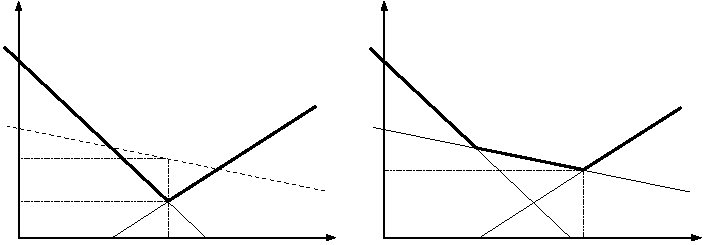
\includegraphics{part_1/chapter_7/figures/Figure4.pdf}};
		\node[right] (zb1_left) at (-5.4, 1) {$(p_k^1)^\top(e_k - C_kx)$};
		\node[left]  (zb2_left) at (0, 0.5) {$(p_k^2)^\top(e_k - C_kx)$};
		\node[right] (zb1_right) at (0.8, 1) {$(p_k^1)^\top(e_k - C_kx)$};
		\node[left]  (zb2_right) at (6.2, 0.5) {$(p_k^2)^\top(e_k - C_kx)$};
		\node[right] (zb3_right) at (4, -1.5) {$(p_k^3)^\top(e_k - C_kx)$};
		\node[right] (zb_opt) at (-2.6, -1.4) {$(p_k^*)^\top(e_k - C_kx)$};
		\node[below] (x1) at (-3.1, -1.9) {$\overline{x}^3$};
		\node[below] (x2) at (3.95, -1.9) {$\overline{x}^4$};
		\node[left]  (theta1) at (-5.6, -1.3) {$\overline{\theta}^3$};
		\node[left]  (theta2) at (0.6, -0.8) {$\overline{\theta}^4$};
		\node[left]  (z_dual) at (-5.6, -0.6) {$z(\overline{x}^3)$};
		\node[below] (x_axis1) at (-0.4, -2) {$x$};
		\node[below] (x_axis2) at (5.8, -2) {$x$};
		\node[right] (z_axis1) at (-5.6, 2) {$z_k(x)$};
		\node[right] (z_axis2) at (0.6, 2) {$z_k(x)$};
	\end{tikzpicture}	
	\caption{$z_k(x)$ is described by 3 line segments. At iteration $l=3$, two are available. The solution to $P_M^3$ returns $\overline{\theta}^3$, which is lower than $z(\overline{x}^3)$, obtained solving $S_k^D$ for $\overline{x}^l$. The solution $p^*_k = p^3_k$ from $z(\overline{x}^l)$ defines the missing segment $(p^*_k)^\top(e_k - C_kx)$. A new optimality cut is added and in iteration $l=4$, $\overline{x}^4$ is obtained from solving $P_M^4$. Notice that we would have $\overline{\theta}^{4} = z(\overline{x}^{4})$, meaning that the algorithm terminates.} \label{p1c7:fig:benders_iteration}
\end{figure}

To identify those violated constraints, first recall that the subproblem (in its primal form) is given by
%
\begin{align*}
	(S_k^l): \mini \ & f^\top y \\
	\st & D_k y_k = e_k - C_k \overline{x}^l \\
	& y_k \geq 0.
\end{align*}
%
Then, two cases can lead to generating violated constraints that must be added to the relaxed primal problem to form $P_M^{l+1}$. The first is when $S_k^l$ is feasible. In that case, a dual optimal basic feasible solution $p^{il}_{k}$ is obtained. If $(p^{il}_k)^\top(e_k - C_k \overline{x}^l) > \overline{\theta}_k^l$, then we can conclude that we just formed a violated constraint of the form of \eqref{p1c7:eq:opt_cut}. The second case is when $S_k^l$ is infeasible, then an extreme ray $w^{rl}_k$ of $P_k$ is available, such that $(w^{rl}_k)^\top(e_k - C_k \overline{x}^l) > 0$, violating \eqref{p1c7:eq:feas_cut}. 

Notice that the above can also be accomplished by solving the dual subproblems $S^D_k$, $k \in \braces{1, \dots, K}$, instead. In that case, the extreme point $p^{il}_k$ is immediately available and so are the extreme rays $w^{rl}_k$ in case of unboundedness.

Algorithm \ref{p1c7:alg:benders} presents a pseudocode for the Benders decomposition. Notice that the method can benefit in terms of efficiency from the use of dual simplex, since we are iteratively adding violated constraints to the relaxed main problem $P_M^l$. Likewise, the dual of the subproblem $S_k^l$, $S_k^{Dl}$ has only the objective function coefficients being modified at each iteration and, in light of the discussion in Section \ref{section_613}, can also benefit from the use of dual simplex. Furthermore, the loop represented by Line \ref{p1c7:alg:benders-loop} can be parallelised to provide further computational performance improvements. 

\begin{algorithm}[H]
    \caption{Benders decomposition} \label{p1c7:alg:benders}
    \begin{algorithmic}[1] %line numbering frequency. 
    \State {\bf initialise.} 
    Let $P_i^l = W_j^l = \emptyset$, for $k \in \braces{1,\dots,K}$, and set
    $l \gets 0$. 
    \Repeat 
        \State solve $P_M^l$ to obtain $\left(\overline{x}^l, \braces{\overline{\theta}_k^l}_{k=1}^K\right)$. 
        \For {$k \in \braces{1,\dots,K}$} \label{p1c7:alg:benders-loop}
            \State solve $S_k^{Dl}$.
            \If{$S_k^{Dl}$ is unbounded} 
            	\State obtain extreme ray $w_j^k$ and make $W^l = W^l \cup \braces{w_j^k}$.
            \Else
            	\State obtain extreme point $p_i^k$ and $P^l = P^l \cup \braces{p_i^k}$
            \EndIf  
        \EndFor
 
        \State $l = l + 1$.        	
    	\Until{$(p^i_k)^\top(e_k - C_k \overline{x}) \leq \overline{\theta}_k, \ \forall k \in \braces{1,\dots,K}$} 
    \State {\bf return} $\left(\overline{x}^l, \braces{\overline{\theta}_k^l}_{k=1}^K\right)$
  \end{algorithmic}
\end{algorithm}

Notice that the algorithm terminates if no violated constraint is found. This in practice implies that $(p^i_k)^\top(e_k - C_k \overline{x}) \leq \overline{\theta}_k$ for all $k \in \braces{1,\dots,K}$, and thus $(\overline{x}, \braces{\overline{\theta}_k}_{k=1}^K)$ is optimal for $P$. In a way, if one considers the dual version subproblem, $S_k^D$, one can notice that it is acting as an implicit search for values of $p^i_k$ that can make $(p^i_k)^\top(e_k - C_k \overline{x})$ larger than $\overline{\theta}_k$, meaning that the current solution $\overline{x}$ violates \eqref{p1c7:eq:opt_cut} and is thus not feasible to $P_M^l$. 

Also, every time one solves $P_M^l$, a dual (lower for minimisation) bound $LB^l = z_{P_M}^l$ is obtained. This is simply because the relaxed main problem is a relaxation of the problem $P$, i.e., it contains less constraints than the original problem $P$. A primal (upper) bound can also be calculated at every iteration, which allows for keeping track of the progress of the algorithm in terms of convergence and preemptively terminate it at any arbitrary optimality tolerance. That can be achieved by setting
%
\begin{align*}
	UB^l &= \min\braces{UB^{l-1}, c^\top \overline{x}^l + \sum_{k=1}^K f^\top \overline{y}_k^l} \\	
	&= \min\braces{UB^{l-1}, z_{P_M}^l - \sum_{k=1}^K \overline{\theta}_k^l + \sum_{k=1}^K z^{Dl}_{k}},
\end{align*}
%
where $(\overline{x}^l, \braces{\overline{\theta}^{l}_k}_{k=1}^K) = \argmin_{x, \theta} \braces{P_M^l}$, $\overline{y}_k^l = \argmin_y \braces{S_k^l}$, and $z^{Dl}_{k}$ is the objective function value of the dual subproblem $S_k^D$ at iteration $l$. Notice that, differently from the lower bound $LB^l$, there are no guarantees that the upper bound $UB^l$ will decrease monotonically. Therefore, one must compare the bound obtained at a given iteration $l$ using the solution $(\overline{x}^l, \overline{y}_1^l,\dots, \overline{y}^l_K)$ against an incumbent (or best-so-far) bound $UB^{l-1}$.

\vfill 

\pagebreak	

\section{Exercises}

\subsection*{Exercise 7.1: Dantzig-Wolfe decomposition}
Consider the following linear programming problem:

\begin{center}
\begin{tabular}{cccccccc}
	 $\mini	$ 	&   		& $-x_{12}$	& 		& 		& $-x_{22}$	& $-x_{23}$	& 		\\
 	 $\st $		& $x_{11}$ 	& $+x_{12}$& $+x_{13}$&		&		&		& = 20   	\\
	 		&		&		&		& $x_{21}$	& $+x_{22}$& $+x_{23}$& = 20   	\\
	 		& $-x_{11}$ 	&		&		& $-x_{21}$	&		& 		& = -20   	\\
			& 		& $-x_{12}$	&		&		& $-x_{22}$	&		& = -10   	\\
			&		&		& $-x_{13}$	&		&		& $-x_{23}$	& = -10   	\\
			& $x_{11}$ 	&		&		& 		& 		& $+x_{23}$& $\le$ 15   	\\
			& $x_{11,}$ 	& $x_{12},$	& $x_{13},$	& $x_{21},$	& $x_{22},$	& $x_{23}$	& $\ge$ 0   	\\
\end{tabular}	
\end{center}

We wish to solve this problem using Dantzig-Wolfe decomposition, where the constraint $x_{11}+x_{23} \le 15$ is the only ``coupling'' constraint and the remaining constraints define a single subproblem.

\begin{itemize}
	\item[(a)] Consider the following two extreme points for the subproblem:
	%
	\begin{equation*}
		x^1 = (20,0,0,0,10,10),		
	\end{equation*}
	%
	and
	\begin{equation*}
		x^2 = (0,10,10,20,0,0).		
	\end{equation*}
	Construct a main problem in which $x$ is constrained to be a convex combination of $x^1$ and $x^2$. Find the optimal primal and dual solutions for the main problem.
	
	\item[(b)] Using the dual variables calculated in part a), formulate the subproblem and find its optimal solution.
	
	\item[(c)] What is the reduced cost of the variable $\lambda_3$ associated with the extreme point $x^3$ obtained from solving the subproblem in part b)?
	
	\item[(d)] Compute a lower bound on the optimal cost.  
	
\end{itemize}




%\subsection*{Exercise 7.2: Cutting stock (CS) problem}
%A paper company has a supply of $P = \{1,\dots,p\}$ large rolls of paper, each of width $W\in \integers_+$. The company has $M = \{1,\dots,m\}$ customers. Each customer $i\in M$ has a demand of $n_i\in \integers_+$ paper stripes of width $w_i \in \integers_+$ with $w_i \leq W$. The company seeks to satisfy customer demands while minimizing the total number of large paper rolls used. We assume that the company has enough rolls $p \in \integers_+$ to satisfy all customer demands. For example, we can assume that

\[
p = \sum_{i\in M} \lceil \frac{n_i}{\lfloor W/w_i \rfloor} \rceil.
\]

This problem is called the Cutting Stock (CS) problem.

\begin{itemize}[itemsep=10pt]
\item[(a)] Formulate the CS as an integer programming problem $IP$ using the following variables:

\begin{enumerate}[itemsep=0pt]
\item $y_j\in \{0,1\}$ for all large paper rolls $j \in P$, with $y_j = 1$ if paper roll $j$ is used and \lb $y_j = 0$ otherwise.
\item $x_{ij} \in \integers_+$ for all customers $i\in M$ and paper rolls $j \in P$, where $x_{ij}$ is equal to the number of stripes of width $w_i$ cut from a large paper roll $j$.
\end{enumerate}

Use two sets of constraints: \emph{demand constraints} imposing that number of stripes cut for each customer $i\in M$ is at least $n_i$, and \emph{capacity constraints} imposing that sum of stripe widths $\sum_{i\in M} w_i x_{ij}$ cut from each paper roll $j\in \{1,\dots,P\}$ is smaller than maximum width $W$.
\item[(b)] Show that the optimal cost $z_{LP}$ of the linear programming relaxation $LP$ of the problem $IP$ in part (a) is

\[
z_{LP} = \frac{\sum_{i\in M} w_i n_i}{W}.
\]
 
\item[(c)] Apply Dantzig-Wolfe reformulation to the problem $IP$ in part (a) with the demand \lb constraints as linking constraints. Write the resulting integer master problem $(IPM)$ and the corresponding \emph{pricing problem} which is used to generate new cutting patterns. 
\item[(d)] Consider a CS problem instance with the following data.
\vspace{5pt}
\begin{enumerate}
 \item Roll width $W = 273$
 \item \textbf{Customer 1}: $w_1 = 18$ ~with $n_1 = 233$
 \item \textbf{Customer 2}: $w_2 = 91$ ~with $n_2 = 310$
 \item \textbf{Customer 3}: $w_3 = 21$ ~with $n_3 = 122$ 
 \item \textbf{Customer 4}: $w_4 = 136$     ~with $n_4 = 157$
 \item \textbf{Customer 5}: $w_5 = 51$ ~with $n_5 = 120$
\end{enumerate}
\vspace{5pt}
Solve the $LP$ relaxation of $IPM$ with this input data with the column generation algorithm. Try to also obtain a feasible solution by rounding the fractional solution. The Julia notebook \href{https://mycourses.aalto.fi/mod/folder/view.php?id=651694}{E101-cutstock.ipynb} has the column generation algorithm readily implemented.
\end{itemize}

\subsection*{Exercise 7.2: Parametric optimization}
Recall the paint factory problem 
%
\begin{align}
	\maxi z = \ & 5x + 4y\\
	\st & 6x + 4y \leq 24\\
	& x + 2y \leq 6 \\
	& y - x \leq  1 \\
	& y \leq 2 \\
	& x, y \geq 0.
\end{align}
%

\begin{itemize} 
    \item[(a)] Formulate a parametric optimization problem $F(x)$, maximizing the profit from selling interior paint ($y$) given the amount of exterior paint ($x$) produced. The solution to this problem must be feasible to the full paint factory problem.
    \item[(b)] Solve the paint factory problem using Benders decomposition. Use $x$ as the main problem variable and $y$ as the subproblem variable.
\end{itemize}

\subsection*{Exercise 7.3: Benders decomposition}
Consider a wholesaler company planning to structure its supply chain to the retailers of a given product. The company needs to distribute the production from many suppliers to a collection of distribution points from which the retailers can collect as much product as they need for a certain period. By default, a pay-as-you-consume contract between wholesaler and retailers is signed and, therefore, the demand at each point is unknown at the moment of shipping. Consider there is no penalty for any unfulfilled demand and any excess must be discarded from one period to the other. The following parameters are given:

\begin{itemize}
	\item $B_i$: production cost at supplier $i$
	\item $C_i$: production capacity at supplier $i$
	\item $D_{js}$: total orders from distribution point $j$ in scenario $s$
	\item $T_{ij}$: transportation cost between $i$ and $j$
	\item $R_j$: revenue for sale at distribution point $j$
	\item $W_j$: disposal cost at distribution point $j$
\end{itemize}

Let the variables be:

\begin{itemize}
	\item $p_i$: production at supplier $i$
	\item $t_{ij}$: amount of products transported between $i$ and $j$
	\item $l_{js}$: amount of products sold from the distribution point $j$ in scenario $s$
	\item $w_{js}$: amount of products discarded from the distribution point $j$ in scenario $s$
	\item $r_j$: amount pre-allocated in the distribution point $j$
\end{itemize}

The model for minimising the cost (considering revenue as a negative cost) is given below,
%
\begin{align*}
	\mini & \sum\limits_{i \in I} B_i p_i + \sum\limits_{i \in I, j \in J} T_{ij} t_{ij} + \sum\limits_{s \in S} P_s \left( \sum\limits_{j \in J} (-R_j l_{js} + W_j w_{js}) \right)                  \\
	 \st & p_i \leq C_i, \                              \forall i \in I                  \\
	     & p_i = \sum\limits_{j \in J}t_{ij}, \         \forall i \in I                  \\
	     & r_j = \sum\limits_{i \in I}t_{ij}, \         \forall j \in J                  \\
	     & r_j = l_{js} + w_{js}, \                     \forall j \in J, \forall s \in S \\
	     & l_{js} \leq D_{js}, \                        \forall j \in J, \forall s \in S \\
	     & p_i \geq 0, \                                \forall i \in I                  \\
	     & r_j \geq 0, \                                \forall j \in J                  \\
	     & t_{ij} \geq 0, \                             \forall i \in I, \forall j \in J \\
	     & l_{js}, w_{js} \geq 0, \                     \forall j \in J, \forall s \in S. 
\end{align*}

Solve an instance of the wholesaler's distribution problem proposed using Benders decomposition. 

